\begin{align*}
  s_{(3,1)}(x_1, x_2, x_3) &=
  \underbrace{x_1^3x_2}_{
  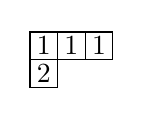
\begin{tikzpicture}[scale=0.35, baseline=-0.5ex]
    \draw (0,0) rectangle (3,1);
    \draw (0,-1) rectangle (1,0);
    \draw (1,-1)--(1,1);
    \draw (2,0)--(2,1);
    \node at (0.5,0.5) {$1$};  \node at (1.5,0.5) {$1$}; \node at (2.5,0.5) {$1$};
    \node at (0.5,-0.5) {$2$};
  \end{tikzpicture}
  }
  +
  \underbrace{x_1^3x_3}_{
  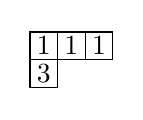
\begin{tikzpicture}[scale=0.35, baseline=-0.5ex]
    \draw (0,0) rectangle (3,1);
    \draw (0,-1) rectangle (1,0);
    \draw (1,-1)--(1,1);
    \draw (2,0)--(2,1);
    \node at (0.5,0.5) {$1$};  \node at (1.5,0.5) {$1$}; \node at (2.5,0.5) {$1$};
    \node at (0.5,-0.5) {$3$};
  \end{tikzpicture}
  }
  +
  \underbrace{x_1^2x_2^2}_{
  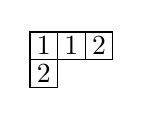
\begin{tikzpicture}[scale=0.35, baseline=-0.5ex]
    \draw (0,0) rectangle (3,1);
    \draw (0,-1) rectangle (1,0);
    \draw (1,-1)--(1,1);
    \draw (2,0)--(2,1);
    \node at (0.5,0.5) {$1$};  \node at (1.5,0.5) {$1$}; \node at (2.5,0.5) {$2$};
    \node at (0.5,-0.5) {$2$};
  \end{tikzpicture}
  }+
  \underbrace{x_1^2x_2x_3}_{
  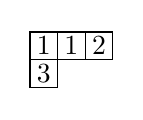
\begin{tikzpicture}[scale=0.35, baseline=-0.5ex]
    \draw (0,0) rectangle (3,1);
    \draw (0,-1) rectangle (1,0);
    \draw (1,-1)--(1,1);
    \draw (2,0)--(2,1);
    \node at (0.5,0.5) {$1$};  \node at (1.5,0.5) {$1$}; \node at (2.5,0.5) {$2$};
    \node at (0.5,-0.5) {$3$};
  \end{tikzpicture}
  }
  +
  \underbrace{x_1^2x_2x_3}_{
  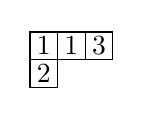
\begin{tikzpicture}[scale=0.35, baseline=-0.5ex]
    \draw (0,0) rectangle (3,1);
    \draw (0,-1) rectangle (1,0);
    \draw (1,-1)--(1,1);
    \draw (2,0)--(2,1);
    \node at (0.5,0.5) {$1$};  \node at (1.5,0.5) {$1$}; \node at (2.5,0.5) {$3$};
    \node at (0.5,-0.5) {$2$};
  \end{tikzpicture}
  }
  +
  \underbrace{x_1^2x_3^3}_{
  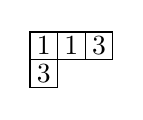
\begin{tikzpicture}[scale=0.35, baseline=-0.5ex]
    \draw (0,0) rectangle (3,1);
    \draw (0,-1) rectangle (1,0);
    \draw (1,-1)--(1,1);
    \draw (2,0)--(2,1);
    \node at (0.5,0.5) {$1$};  \node at (1.5,0.5) {$1$}; \node at (2.5,0.5) {$3$};
    \node at (0.5,-0.5) {$3$};
  \end{tikzpicture}
  }
  +
  \underbrace{x_1x_2^3}_{
  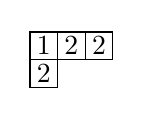
\begin{tikzpicture}[scale=0.35, baseline=-0.5ex]
    \draw (0,0) rectangle (3,1);
    \draw (0,-1) rectangle (1,0);
    \draw (1,-1)--(1,1);
    \draw (2,0)--(2,1);
    \node at (0.5,0.5) {$1$};  \node at (1.5,0.5) {$2$}; \node at (2.5,0.5) {$2$};
    \node at (0.5,-0.5) {$2$};
  \end{tikzpicture}
  }
  +
  \underbrace{x_1x_2^2x_3}_{
  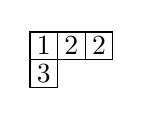
\begin{tikzpicture}[scale=0.35, baseline=-0.5ex]
    \draw (0,0) rectangle (3,1);
    \draw (0,-1) rectangle (1,0);
    \draw (1,-1)--(1,1);
    \draw (2,0)--(2,1);
    \node at (0.5,0.5) {$1$};  \node at (1.5,0.5) {$2$}; \node at (2.5,0.5) {$2$};
    \node at (0.5,-0.5) {$3$};
  \end{tikzpicture}
  } \\
  &\hspace{1cm}+
  \underbrace{x_1x_2^2x_3}_{
  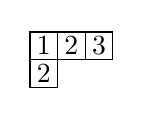
\begin{tikzpicture}[scale=0.35, baseline=-0.5ex]
    \draw (0,0) rectangle (3,1);
    \draw (0,-1) rectangle (1,0);
    \draw (1,-1)--(1,1);
    \draw (2,0)--(2,1);
    \node at (0.5,0.5) {$1$};  \node at (1.5,0.5) {$2$}; \node at (2.5,0.5) {$3$};
    \node at (0.5,-0.5) {$2$};
  \end{tikzpicture}
  }
  +
  \underbrace{x_1x_2x_3^2}_{
  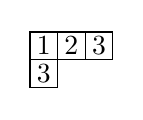
\begin{tikzpicture}[scale=0.35, baseline=-0.5ex]
    \draw (0,0) rectangle (3,1);
    \draw (0,-1) rectangle (1,0);
    \draw (1,-1)--(1,1);
    \draw (2,0)--(2,1);
    \node at (0.5,0.5) {$1$};  \node at (1.5,0.5) {$2$}; \node at (2.5,0.5) {$3$};
    \node at (0.5,-0.5) {$3$};
  \end{tikzpicture}
  }
  +
  \underbrace{x_1x_2x_3^2}_{
  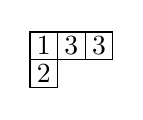
\begin{tikzpicture}[scale=0.35, baseline=-0.5ex]
    \draw (0,0) rectangle (3,1);
    \draw (0,-1) rectangle (1,0);
    \draw (1,-1)--(1,1);
    \draw (2,0)--(2,1);
    \node at (0.5,0.5) {$1$};  \node at (1.5,0.5) {$3$}; \node at (2.5,0.5) {$3$};
    \node at (0.5,-0.5) {$2$};
  \end{tikzpicture}
  }
  +
  \underbrace{x_1x_3^3}_{
  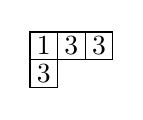
\begin{tikzpicture}[scale=0.35, baseline=-0.5ex]
    \draw (0,0) rectangle (3,1);
    \draw (0,-1) rectangle (1,0);
    \draw (1,-1)--(1,1);
    \draw (2,0)--(2,1);
    \node at (0.5,0.5) {$1$};  \node at (1.5,0.5) {$3$}; \node at (2.5,0.5) {$3$};
    \node at (0.5,-0.5) {$3$};
  \end{tikzpicture}
  }
  +
  \underbrace{x_2^3x_3}_{
  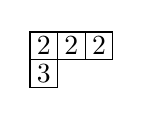
\begin{tikzpicture}[scale=0.35, baseline=-0.5ex]
    \draw (0,0) rectangle (3,1);
    \draw (0,-1) rectangle (1,0);
    \draw (1,-1)--(1,1);
    \draw (2,0)--(2,1);
    \node at (0.5,0.5) {$2$};  \node at (1.5,0.5) {$2$}; \node at (2.5,0.5) {$2$};
    \node at (0.5,-0.5) {$3$};
  \end{tikzpicture}
  }
  +
  \underbrace{x_2^2x_3^2}_{
  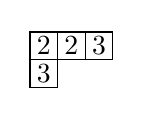
\begin{tikzpicture}[scale=0.35, baseline=-0.5ex]
    \draw (0,0) rectangle (3,1);
    \draw (0,-1) rectangle (1,0);
    \draw (1,-1)--(1,1);
    \draw (2,0)--(2,1);
    \node at (0.5,0.5) {$2$};  \node at (1.5,0.5) {$2$}; \node at (2.5,0.5) {$3$};
    \node at (0.5,-0.5) {$3$};
  \end{tikzpicture}
  }
  +
  \underbrace{x_2x_3^3}_{
  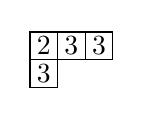
\begin{tikzpicture}[scale=0.35, baseline=-0.5ex]
    \draw (0,0) rectangle (3,1);
    \draw (0,-1) rectangle (1,0);
    \draw (1,-1)--(1,1);
    \draw (2,0)--(2,1);
    \node at (0.5,0.5) {$2$};  \node at (1.5,0.5) {$3$}; \node at (2.5,0.5) {$3$};
    \node at (0.5,-0.5) {$3$};
  \end{tikzpicture}
  }
  \\
  &= x_1^3x_2 + x_1^3x_3 + x_1^2x_2^2 + 2x_1^2x_2x_3 + x_1^2x_2^2 + x_1x_2^3 + 2x_1x_2^2x_3 \\
  &\hspace{1cm}+ 2x_1x_2x_3^2 + x_1x_3^3 + x_2^3x_3 + x_2^2x_3^2 + x_2x_3^3 + x_2x_3^3 \\
  &= m_{(3,1)} + 2m_{(2,1,1)} + m_{(2,2)}
\end{align*}